\documentclass[a4paper]{extarticle}
\usepackage{graphicx}
\usepackage[a4paper]{geometry}
\usepackage{amsmath}
\usepackage{amssymb}
\usepackage{hyperref}
\usepackage[utf8]{inputenc}
\usepackage[T1]{fontenc}
\usepackage{tikz}
\usepackage{listings}
\usepackage{blkarray}
\usepackage{color}
\usepackage{caption}
\usepackage{subcaption}
 
\definecolor{codegreen}{rgb}{0,0.6,0}
\definecolor{codegray}{rgb}{0.5,0.5,0.5}
\definecolor{codepurple}{rgb}{0.58,0,0.82}
\definecolor{backcolour}{rgb}{0.95,0.95,0.92}
 
\lstdefinestyle{mystyle}{
    backgroundcolor=\color{backcolour},   
    commentstyle=\color{codegreen},
    keywordstyle=\color{magenta},
    numberstyle=\tiny\color{codegray},
    stringstyle=\color{codepurple},
    basicstyle=\footnotesize,
    breakatwhitespace=false,         
    breaklines=true,                 
    captionpos=b,                    
    keepspaces=true,                 
    numbers=left,                    
    numbersep=5pt,                  
    showspaces=false,                
    showstringspaces=false,
    showtabs=false,                  
    tabsize=2
}
 
\lstset{
	style=mystyle,
	frame=single	
}


\setlength\parindent{0pt}

\makeatletter
\renewcommand*\env@matrix[1][*\c@MaxMatrixCols c]{%
  \hskip -\arraycolsep
  \let\@ifnextchar\new@ifnextchar
  \array{#1}}
\makeatother

\newcommand*{\putunder}[2]{%
  {\mathop{#1}_{\textstyle #2}}%
}

\newcommand{\stirling}[2]{\genfrac{}{}{0pt}{0}{#1}{#2}}

\newcommand{\R}{\mathbb{R}}

\title{Project 1 INF236}
\author{Markus Ragnhildstveit, hef005}

\begin{document}

\maketitle

\tableofcontents
\newpage

I decided to run the performance tests on my computer, because the results I got on lyng was so inconsistent. My computer has 4 cores with 2 hyperthreads on each core. So a total of 8 hyperthreads.

\section{1D}
\begin{figure}[!h]
	\center
	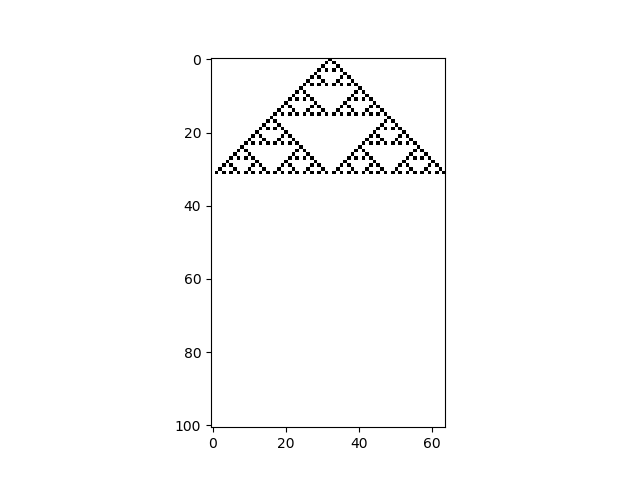
\includegraphics[scale=1.0]{Sequential.png}
	\caption{100 iteration with $0^{32}10^{31}$ as initial configuration.}
\end{figure}

\subsection{How to run the program}
To run the sequential program, it needs the following arguments: rulefile kx.txt numOfIt. Where rulefile can be any rulefile, but the only available is mod2.txt. Also x in kx.txt can be 10, 11, 12, 13, 14, 15, 16, 17, 18, 19 or 20. E.g. k10.txt. numOfIt is the number of iterations, which can be any number over 0.

To run the parallel program, it needs the following arguments: rulefile kx.txt numOfIt. Where rulefile can be any rulefile, but the only available is mod2.txt. Also x in kx.txt can be 10, 11, 12, 13, 14, 15, 16, 17, 18, 19 or 20. E.g. k10.txt. numOfIt is the number of iterations, which can be any number over 0.
\subsection{Table}
\begin{center}
  \begin{tabular}{ c | | c | c | c | c | c | c | c | c | }
  	k\textbackslash  n & 1 & 2 & 4 & 8 & 16 & 32 & 64 & 128 \\ \hline
    \hline
    10 & 2.14s & 1.58s & 1.84s & 2.16s & 3.69s & 5.89s & 10.52s & 21.96s \\ \hline 
    11 & 3.83s & 3.26s & 3.09s & 3.86s & 5.46s & 7.47s & 12.73s & 24.79s \\ \hline 
    12 & 9.39s & 6.95s & 6.73s & 7.55s & 9.32s & 11.17s & 16.84s & 30.2s \\ \hline 
    13 & 27.27s & 17.3s & 16.58s & 18.14s & 19.59s & 35.68s & 30.84s & 51.16s \\
    \hline
  \end{tabular}
\end{center}

When running with 100000 iterations, I was not able to run with k larger than 13 because of limited memory. So I decided to run only 1000 iterations when k was larger than 13.

\begin{center}
  \begin{tabular}{ c | | c | c | c | c | c | c | c | c | }
  	k\textbackslash  n & 1 & 2 & 4 & 8 & 16 & 32 & 64 & 128 \\ \hline
    \hline
    14 & 0.28s & 0.22s & 0.22s & 0.28s & 0.29s & 0.32s & 0.44s & 0.66s \\ \hline 
    15 & 0.56s & 0.44s & 0.42s & 0.49s & 0.53s & 0.59s & 0.72s & 1.05s \\ \hline 
    16 & 1.14s & 0.87s & 0.87s & 1.02s & 1.04s & 1.32s & 1.38s & 1.82s \\ \hline 
    17 & 3.22s & 1.85s & 1.88s & 2.2s & 2.17s & 2.49s & 2.41s & 3.33s \\ \hline 
    18 & 5.28s & 4.81s & 3.59s & 4.19s & 4.36s & 4.4s & 4.73s & 6.87s \\ \hline 
    19 & 12.08s & 8.81s & 9.59s & 9.85s & 9.41s & 9.68s & 10.78s & 14.02s \\ \hline 
    20 & 39.32s & 22.54s & 21.39s & 23.48s & 25.1s & 24.73s & 25.62s & 33.54s \\
    \hline
  \end{tabular}
\end{center}

I noticed that the antivirus started to process when the data started, so this may have affected the results.
We can however see that the optimal number of processes is close to the number of cores my machine has. I noticed that the gather function was what made 2 processes almost as fast as 4 or 8 processes, since with 2 there is less time consumption with fewer processes. I took the time before and after gather, called time1 and time2, which you can find in the result1D.csv.

\subsection{How I parallelized my program}
To parallelize my 1D program I first had to get the initial config and lookup table. this is done only in process 1 to avoid multiple reads to files. Then process 1 needs to calculate how big part of the config each process will get. This is done by dividing the number of cells in the config by the number of processes, but also by looking at the rest. To send each process a part of the config, I use MPI\_ Scatterv.

When running each iteration each process will send and receive the neighbouring cells so their local config can  be calculated. This is done by making even numbered processes send first and odd numbered receive first.

In the start when I gathered, I had a for-loop which gathered each iteration independently, but I noticed this took very long time when the number of processes increased. I then change to only using 1 gather, but the data became unorganized. To fix this when e.g. reading to a file, I had to locate the index which was the start for each process's history. You can find this in the writeToFile function.

\section{2D}
\subsection{How to run}
To run the sequential program, it needs the arguments as follow: gameOfLife.txt config\_n.txt numOfIt. Where n is the size of n, the only supported n for this program is 3, 5, 20 and 1024. And where numOfIt is the number of iterations, which can be any number over 0.

To run the parallel program, it needs the arguments as follow: gameOfLife.txt n numOfIt. Where n is the size of the config. it can be any integer over 3, since it gets generated in the program. numOfIt is the number of iterations, it can be any number over 0. 
\subsection{How I parallelized my program}
I wanted it to work for any combination of n and p, so I decided to use Scatterv and Gatherv as I did in 1D. Instead of dividing the number of cells, I divided the height between the processes, so that it would be easier to send and receive when running the iterations. The reason I divided the height instead of the width, was that then only 1 scatter was necessary.

When running each iteration, send and receive the first and last row with the corresponding neighbour. To avoid deadlock, I make the even number processes send first and then receive, while odd number number processes will receive first and the send. If there is an odd number of processes, process 0 has to receive first from process n-1 to avoid deadlock.
To get neighbours of a cell, I check the row position +-1 and column position +-1. If the row is either first or last, some of the neighbours needs to be find from the array which saves the data received from neighbouring processes.

When gathering the configuration together again, it can be done the same way it is scattered.

\begin{figure}[h!]
\centering
\begin{subfigure}{.5\textwidth}
  \centering
  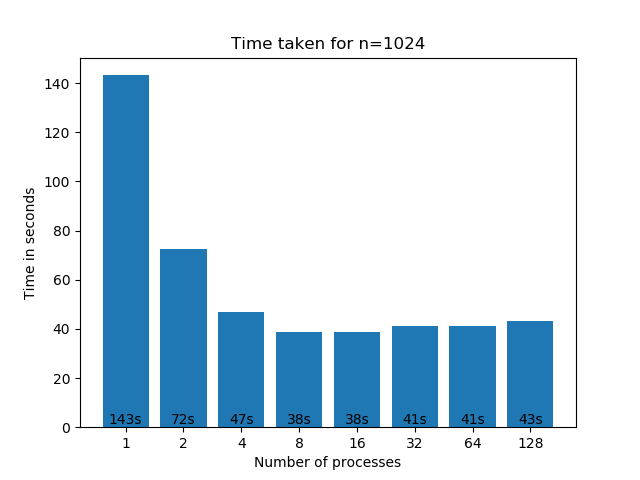
\includegraphics[width=1.1\linewidth]{../Plot/bar1024.png}
\end{subfigure}%
\begin{subfigure}{.5\textwidth}
  \centering
  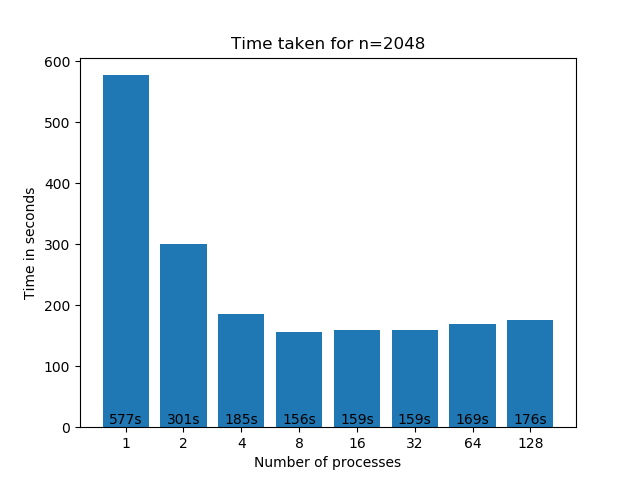
\includegraphics[width=1.1\linewidth]{../Plot/bar2048.png}
\end{subfigure}
\end{figure}

\begin{figure}[h!]
\centering
\begin{subfigure}{.5\textwidth}
  \centering
  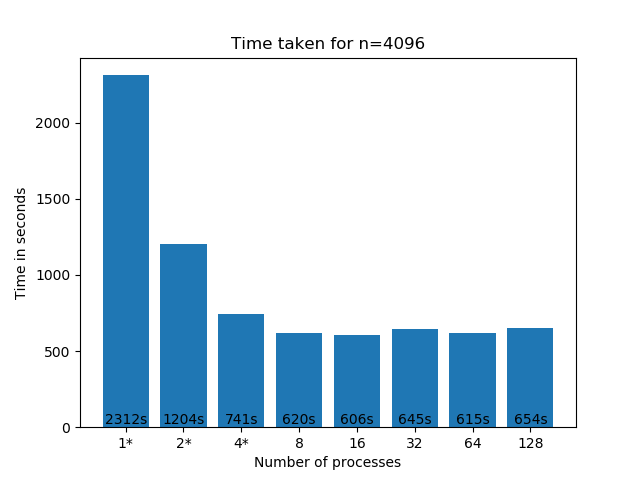
\includegraphics[width=1.1\linewidth]{../Plot/bar4096.png}
\end{subfigure}%
\begin{subfigure}{.5\textwidth}
  \centering
  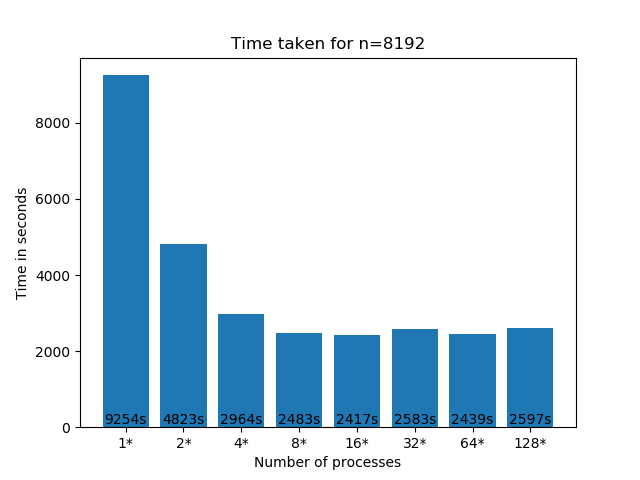
\includegraphics[width=1.1\linewidth]{../Plot/bar8192.png}
\end{subfigure}
\end{figure}

Numbers with a star * is estimation using linear regression using execution time from both less iterations and smaller n. I do this because i noticed it was a linearly increasing in time used when I look at the number of elements processed (n*n) and number of iterations. It looks like the model thinks that processes with more than 8 will be faster when n is increasing, but this is likely only noise. We can see that 8 processes is the fastest for the real data I have. This corresponds to the number of hyperthreads my machine has, which has 4 cores and 2 hyperthreads per core.

Looking at larger values for n is going to take unnecessary long time, with 1 process and n=65536 estimated to use 164.5 hours to complete.

The data used to create the bars are in the table under:
\begin{center}
  \begin{tabular}{ c | | c | c | c | c | c | c | c | c | }
  	 & 1 & 2 & 4 & 8 & 16 & 32 & 64 & 128 \\ \hline
    \hline
    1024 & 2.39m & 1.21m & 47.03s & 38.6s & 38.65s & 41.37s & 41.25s & 43.26s\\ \hline 
    2048 & 9.62m & 5.03m & 3.1m & 2.6m & 2.66m & 2.65m & 2.83m & 2.95m\\ \hline 
    4096 & 38.54m* & 20.08m* & 12.36m* & 10.35m & 10.11m & 10.76m & 10.26m & 10.9m\\ \hline 
    8192 & 2.57h* & 1.34h* & 49.4m* & 41.39m* & 40.29m* & 43.06m* & 40.66m* & 43.29m*\\ \hline 
    16384 & 10.28h* & 5.36h* & 3.29h* & 2.76h* & 2.68h* & 2.87h* & 2.7h* & 2.88h*\\ \hline 
    32768 & 41.14h* & 21.44h* & 13.17h* & 11.04h* & 10.73h* & 11.48h* & 10.8h* & 11.51h*\\ \hline 
    65536 & 164.54h* & 85.78h* & 52.68h* & 44.14h* & 42.9h* & 45.94h* & 43.2h* & 46.03h* \\
    \hline
  \end{tabular}
\end{center}

The raw data can be found in report.csv. 

\section{Branching}
I felt like it was hard to understand how the program should work without example, but I implemented with some assumptions that I thought was correct.

\subsection{How to run}
To run the sequential program, it needs the following arguments: rulefile a. Where rulefile is any file with rules, but the only available file is branchingmod3.txt. And a is the binary string, e.g. 1010 when branchingmod3.txt is used.

To run the parallel program, it needs the following arguments: rulefile a. Where rulefile is any file with rules, but the only available file is branchingmod3.txt. And a is the binary string, e.g. 1010 when branchingmod3.txt is used. It is possible to run the program with generating if you uncomment line 40, 60 and 61. And comment out line 42, 58 and 59.

\subsection{Problem 2}
The reason that it is possible to compute val(P, a) is that the operation is associative, so the result could be calculated in this order for an example with size 8:

\begin{figure}[!h]
	\centering
	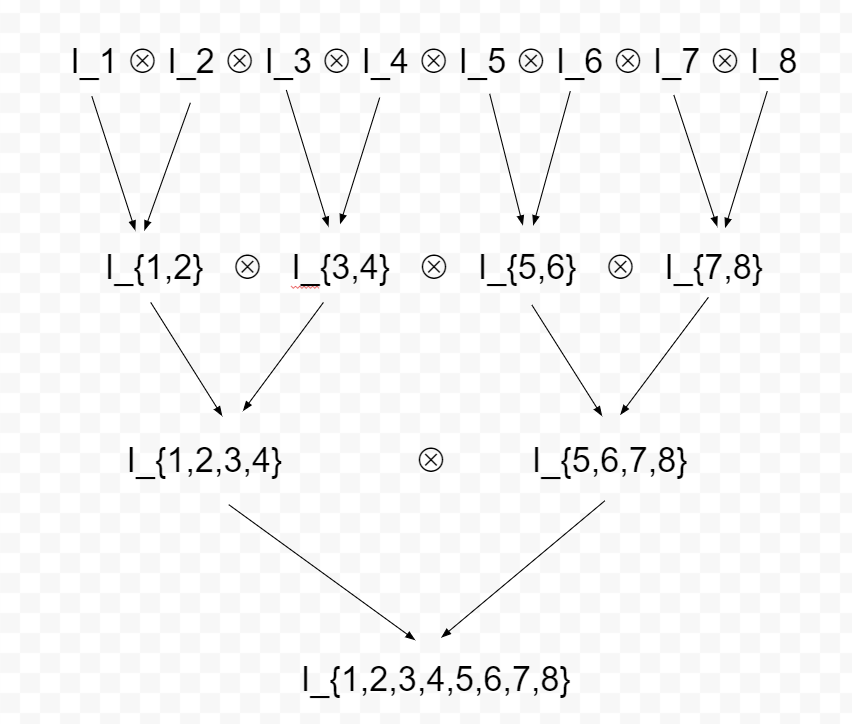
\includegraphics[scale=0.5]{Problemset_1_P3_2.png}
\end{figure}

As we can see the problem length halves each iteration. In the first iteration needs 4 processes which has 2 numbers each. Next iteration 2 processes is needed, and last only 1 process is needed. Since the problem halves each iteration, it will finish in $O(log_2(m)) = O(log(m))$ time.

\subsection{How I parallelized my program}
To parallelize the program, I made process 0 parse the rule file and convert the assignment argument to an int array. The rules with their sizes was broadcasted to all processes. I then scattered the array between each process with scatterv. First each process calculates the result of its own array. 

To calculate the results each processed had with each other, I used MPI\_Reduce. To reduce I needed to create my own MPI operation (similar to how MPI\_SUM works in the background). This function is called valmpi. In this function, the only way to also receive the operation lookup table, I needed to merge the result and operation lookuptable into 1 array, and send it into the MPI\_Reduce function. So when MPI\_Reduce was done, the end result would be the first element in the received array.

I do have a bug in the parallel program when using the operation lookup table, but I did not have time to fix it.



\end{document}
